\newpage
\thispagestyle{empty}
\appendix
\renewcommand{\thechapter}{\arabic{chapter}}
\renewcommand{\thesection}{\thechapter.\arabic{section}}
\renewcommand{\thesubsection}{\thechapter.\arabic{section}.\arabic{subsection}}
\addcontentsline{toc}{chapter}{LAMPIRAN}
\chapter{DATASET}
\label{lampiran1}
\section{Nama dan Koordinat SMA di Kabupaten Probolinggo}

{\scriptsize
\begin{longtable}[c]{clcc}
\cline{2-4}
\rowcolor[HTML]{4472C4} 
{\color[HTML]{FFFFFF} \textbf{No.}} &
  \multicolumn{1}{c}{\cellcolor[HTML]{4472C4}{\color[HTML]{FFFFFF} \textbf{Nama Sekolah}}} &
  \multicolumn{1}{c}{\cellcolor[HTML]{4472C4}{\color[HTML]{FFFFFF} \textbf{\begin{tabular}[c]{@{}c@{}}Latitude\\      (Sumbu X)\end{tabular}}}} &
  \multicolumn{1}{c}{\cellcolor[HTML]{4472C4}{\color[HTML]{FFFFFF} \textbf{\begin{tabular}[c]{@{}c@{}}Longitude\\      (Sumbu Y)\end{tabular}}}} \\ \cline{2-4} 
\endhead
%
\cline{2-4}
\endfoot
%
\endlastfoot
%
\rowcolor[HTML]{D9E1F2} 
1  & SMA DARUL HIKMAH                      & -7,76 & 113,43 \\
2  & SMA   DARUT TAQWA                     & -7,79 & 113,53 \\
\rowcolor[HTML]{D9E1F2} 
3  & SMA HAYATUL ISLAM                     & -7,88 & 113,43 \\
4  & SMA   IRSYADUL MUBTADIIN              & -7,83 & 113,42 \\
\rowcolor[HTML]{D9E1F2} 
5  & SMA ISLAM AR ROFIIYAH                 & -7,77 & 113,41 \\
6  & SMA   ISLAM MIFTAHUL ULUM GUNUNG GENI & -7,86 & 113,29 \\
\rowcolor[HTML]{D9E1F2} 
7  & SMA ISLAM SYARIF HIDAYATULLAH         & -7,81 & 113,51 \\
8  & SMA   ISTIQLAL                        & -7,78 & 113,51 \\
\rowcolor[HTML]{D9E1F2} 
9  & SMA NAZHATUT THOLIBIN                 & -7,84 & 113,30 \\
10 & SMA   NEGERI 1 DRINGU                 & -7,75 & 113,24 \\
\rowcolor[HTML]{D9E1F2} 
11 & SMA NEGERI 1 KURIPAN                  & -7,89 & 113,14 \\
12 & SMA   NEGERI 1 MARON                  & -7,84 & 113,36 \\
\rowcolor[HTML]{D9E1F2} 
13 & SMA NEGERI 1 SUMBERASIH               & -7,74 & 113,13 \\
14 & SMA   NEGERI 2 KRAKSAAN               & -7,73 & 113,46 \\
\rowcolor[HTML]{D9E1F2} 
15 & SMA PLUS AL KHOLILIYAH                & -7,81 & 113,34 \\
16 & SMA   SIROJUL ARIFIN                  & -7,80 & 113,42 \\
\rowcolor[HTML]{D9E1F2} 
17 & SMA TARUNA DRA. ZULAEHA               & -7,85 & 113,23 \\
18 & SMA   TERPADU DARUT TAUHID            & -7,81 & 113,40 \\
\rowcolor[HTML]{D9E1F2} 
19 & SMA UNGGULAN BADRIDDUJA               & -7,75 & 113,42 \\
20 & SMA   Zainal Abidin                   & -7,89 & 113,34 \\
\rowcolor[HTML]{D9E1F2} 
21 & SMAN 1 BANTARAN                       & -7,84 & 113,18 \\
22 & SMAN 1   BESUK                        & -7,83 & 113,50 \\
\rowcolor[HTML]{D9E1F2} 
23 & SMAN 1 GADING                         & -7,87 & 113,37 \\
24 & SMAN 1   GENDING                      & -7,81 & 113,32 \\
\rowcolor[HTML]{D9E1F2} 
25 & SMAN 1 KRAKSAAN                       & -7,76 & 113,42 \\
26 & SMAN 1   KRUCIL                       & -7,94 & 113,48 \\
\rowcolor[HTML]{D9E1F2} 
27 & SMAN 1 LECES                          & -7,87 & 113,25 \\
28 & SMAN 1   PAITON                       & -7,72 & 113,51 \\
\rowcolor[HTML]{D9E1F2} 
29 & SMAN 1 SUKAPURA                       & -7,89 & 113,05 \\
30 & SMAN 1   SUMBER                       & -7,94 & 113,11 \\
\rowcolor[HTML]{D9E1F2} 
31 & SMAN 1 TIRIS                          & -7,97 & 113,40 \\
32 & SMAN 1   TONGAS                       & -7,74 & 113,10 \\
\rowcolor[HTML]{D9E1F2} 
33 & SMAS ADDASUQI                         & -7,83 & 113,30 \\
34 & SMAS AL   HASYIMI                     & -7,79 & 113,57 \\
\rowcolor[HTML]{D9E1F2} 
35 & SMAS AL KHAIRIYAH                     & -7,75 & 113,43 \\
36 & SMAS   ASSUBHAN                       & -7,75 & 113,16 \\
\rowcolor[HTML]{D9E1F2} 
37 & SMAS DARUL AKHLAQ                     & -7,77 & 113,14 \\
38 & SMAS   DARUL MUKHLASHIN               & -7,85 & 113,26 \\
\rowcolor[HTML]{D9E1F2} 
39 & SMAS DARUL ULUM                       & -7,93 & 113,33 \\
40 & SMAS   HAYATUL ISLAM                  & -7,83 & 113,43 \\
\rowcolor[HTML]{D9E1F2} 
41 & SMAS IHYAUL IMAN                      & -7,88 & 113,45 \\
42 & SMAS   ISLAM AR ROHMAH                & -7,93 & 113,58 \\
\rowcolor[HTML]{D9E1F2} 
43 & SMAS ISLAM IRTIQOIYAH                 & -7,79 & 113,40 \\
44 & SMAS   ISLAM KHAIRIYAH                & -7,88 & 113,50 \\
\rowcolor[HTML]{D9E1F2} 
45 & SMAS ISLAM MAMBAUL ULUM               & -7,85 & 113,42 \\
46 & SMAS   ISLAM MIFTAHUL AFKAR           & -7,75 & 113,43 \\
\rowcolor[HTML]{D9E1F2} 
47 & SMAS ISLAM MIFTAHUL ARIFIN            & -7,86 & 113,18 \\
48 & SMAS   ISLAM MIFTAHUL ULUM JATIURIP   & -7,80 & 113,39 \\
\rowcolor[HTML]{D9E1F2} 
49 & SMAS ISLAM MIFTAHUL ULUM OPO OPO      & -7,83 & 113,41 \\
50 & SMAS   ISLAM NURUL HUDA               & -7,94 & 113,53 \\
\rowcolor[HTML]{D9E1F2} 
51 & SMAS ISLAM NURUR RIYADLAH             & -7,74 & 113,48 \\
52 & SMAS   ISLAM RADEN FATAH              & -7,84 & 113,32 \\
\rowcolor[HTML]{D9E1F2} 
53 & SMAS ISLAM RAUDLATUL KHAIR            & -7,79 & 113,34 \\
54 & SMAS   ISLAM SIROJUL UMMAH            & -7,84 & 113,48 \\
\rowcolor[HTML]{D9E1F2} 
55 & SMAS ISLAM SUMBERASIH                 & -7,79 & 113,17 \\
56 & SMAS   ISLAM TAJUNG SARI              & -7,74 & 113,13 \\
\rowcolor[HTML]{D9E1F2} 
57 & SMAS ISLAM TERPADU ULIL ALBAB         & -7,79 & 113,34 \\
58 & SMAS   ISLAM ULUL ALBAB               & -7,86 & 113,35 \\
\rowcolor[HTML]{D9E1F2} 
59 & SMAS ISLAM ZAINUL HIKAM               & -7,84 & 113,22 \\
60 & SMAS IT   KYAI SEKAR AL AMRI          & -7,84 & 113,22 \\
\rowcolor[HTML]{D9E1F2} 
61 & SMAS MIFTAHUL HASANAIN                & -7,81 & 113,40 \\
62 & SMAS   MUHAMMAD SHODIQ                & -7,83 & 113,37 \\
\rowcolor[HTML]{D9E1F2} 
63 & SMAS MUHAMMADIYAH 3 PROBOLINGGO       & -7,82 & 113,32 \\
64 & SMAS   NURUL HASAN                    & -7,93 & 113,31 \\
\rowcolor[HTML]{D9E1F2} 
65 & SMAS NURUL IMAN                       & -7,86 & 113,41 \\
66 & SMAS   NURUL JADID                    & -7,71 & 113,50 \\
\rowcolor[HTML]{D9E1F2} 
67 & SMAS SA ADAH NIZHAMUL ISLAM           & -7,85 & 113,35 \\
68 & SMAS   SYECH ABD QODIR ZAELANI        & -7,77 & 113,43 \\
\rowcolor[HTML]{D9E1F2} 
69 & SMAS TAMAN MADYA                      & -7,77 & 113,41 \\
70 & SMAS   TUNAS LUHUR                    & -7,73 & 113,52 \\
\rowcolor[HTML]{D9E1F2} 
71 & SMAS UNGGULAN HAF-SA Z H              & -7,79 & 113,38 \\
72 & SMAS   WALI SONGO                     & -7,78 & 113,17 \\
\rowcolor[HTML]{D9E1F2} 
73 & SMAS ZAINUL HASAN 1                   & -7,79 & 113,38 \\
74 & SMAS   ZAINUL HASAN 2 KRUCIL          & -7,96 & 113,49 \\
\rowcolor[HTML]{D9E1F2} 
75 & SMASI NURUL HIDAYAH                   & -7,81 & 113,40 \\ \cline{2-4} 
\end{longtable}
}

\chapter{HASIL KLASTER}
\label{lampiran2}

\section{Pengelompokan 2 klaster}

\subsection{Klaster A}
\begin{table}[H]
\scriptsize
\centering
\begin{tabular}{lcc}
\rowcolor[HTML]{4472C4} 
{\color[HTML]{FFFFFF} \textbf{Nama   Sekolah}} & {\color[HTML]{FFFFFF} \textbf{Latitude (Sumbu X)}} & {\color[HTML]{FFFFFF} \textbf{Longitude (Sumbu Y)}} \\
\rowcolor[HTML]{D9E1F2} 
SMA ISLAM MIFTAHUL ULUM GUNUNG   GENI & -7,86 & 113,29 \\
SMA   NAZHATUT THOLIBIN               & -7,84 & 113,30 \\
\rowcolor[HTML]{D9E1F2} 
SMA NEGERI 1 DRINGU                   & -7,75 & 113,24 \\
SMA   NEGERI 1 KURIPAN                & -7,89 & 113,14 \\
\rowcolor[HTML]{D9E1F2} 
SMA NEGERI 1 SUMBERASIH               & -7,74 & 113,13 \\
SMA   TARUNA DRA. ZULAEHA             & -7,85 & 113,23 \\
\rowcolor[HTML]{D9E1F2} 
SMAN 1 BANTARAN                       & -7,84 & 113,18 \\
SMAN   1 GENDING                      & -7,81 & 113,32 \\
\rowcolor[HTML]{D9E1F2} 
SMAN 1 LECES                          & -7,87 & 113,25 \\
SMAN   1 SUKAPURA                     & -7,89 & 113,05 \\
\rowcolor[HTML]{D9E1F2} 
SMAN 1 SUMBER                         & -7,94 & 113,11 \\
SMAN   1 TONGAS                       & -7,74 & 113,10 \\
\rowcolor[HTML]{D9E1F2} 
SMAS ADDASUQI                         & -7,83 & 113,30 \\
SMAS   ASSUBHAN                       & -7,75 & 113,16 \\
\rowcolor[HTML]{D9E1F2} 
SMAS DARUL AKHLAQ                     & -7,77 & 113,14 \\
SMAS   DARUL MUKHLASHIN               & -7,85 & 113,26 \\
\rowcolor[HTML]{D9E1F2} 
SMAS DARUL ULUM                       & -7,93 & 113,33 \\
SMAS   ISLAM MIFTAHUL ARIFIN          & -7,86 & 113,18 \\
\rowcolor[HTML]{D9E1F2} 
SMAS ISLAM RADEN FATAH                & -7,84 & 113,32 \\
SMAS   ISLAM SUMBERASIH               & -7,79 & 113,17 \\
\rowcolor[HTML]{D9E1F2} 
SMAS ISLAM TAJUNG SARI                & -7,74 & 113,13 \\
SMAS   ISLAM ZAINUL HIKAM             & -7,84 & 113,22 \\
\rowcolor[HTML]{D9E1F2} 
SMAS IT KYAI SEKAR AL AMRI            & -7,84 & 113,22 \\
SMAS   MUHAMMADIYAH 3 PROBOLINGGO     & -7,82 & 113,32 \\
\rowcolor[HTML]{D9E1F2} 
SMAS NURUL HASAN                      & -7,93 & 113,31 \\
SMAS   WALI SONGO                     & -7,78 & 113,17
\end{tabular}
\end{table}

%\newpage
%\thispagestyle{empty}
%\section*{Lampiran 2 Instrumen Penelitian}

%\begin{enumerate}
%\item Jupyter Notebook

%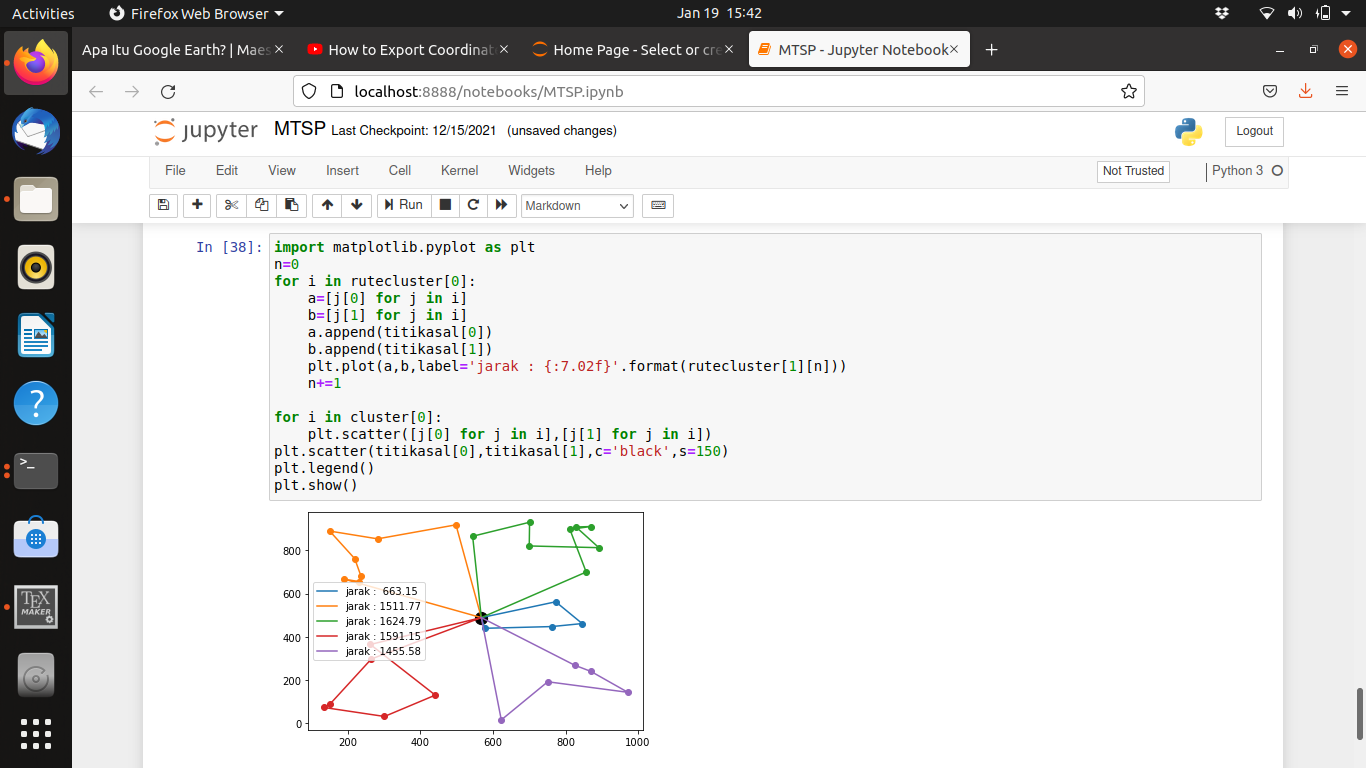
\includegraphics[width=13cm]{instrumen2.png}

%\item Google Earth

%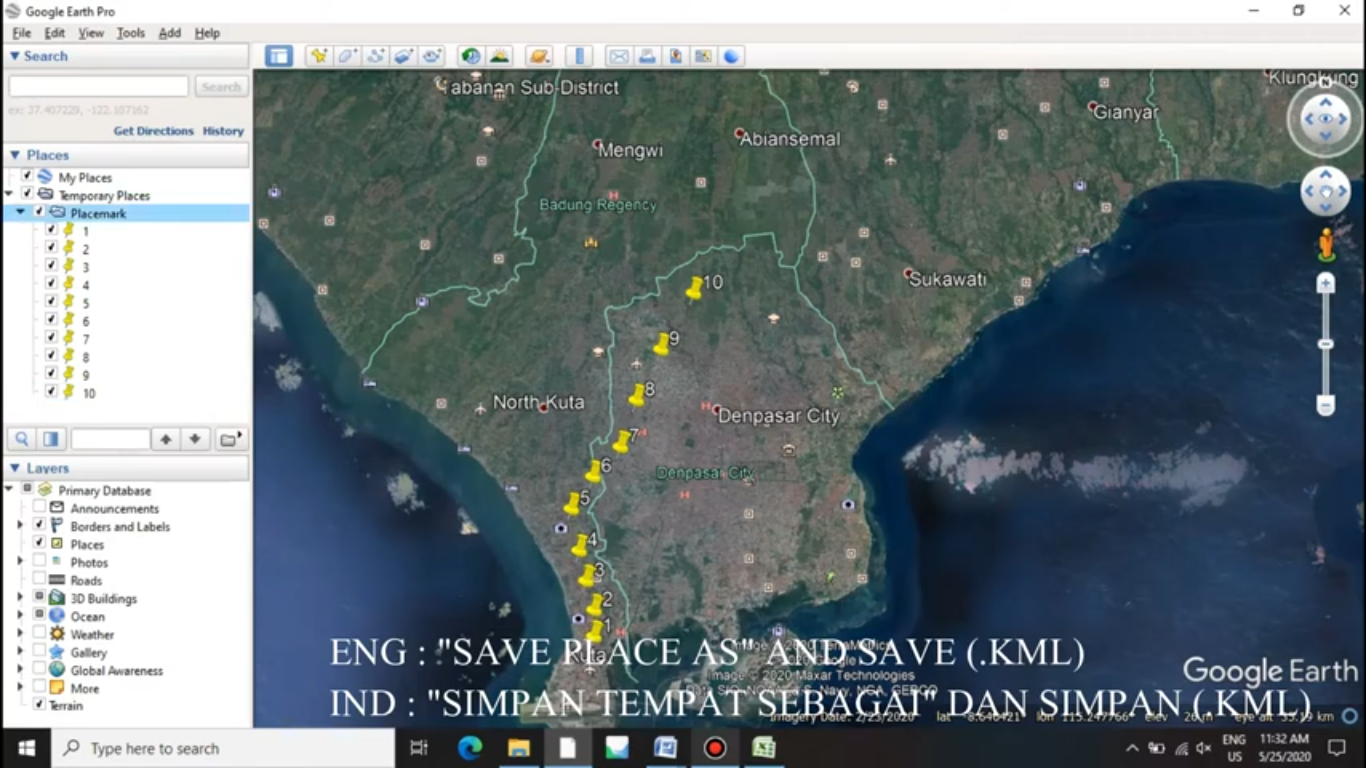
\includegraphics[width=13cm]{instrumen1.png}

%\end{enumerate}